\section{Komplementärfilter für die Winkel $\bs{\varphi}$}
Im Rahmen der Vorarbeit hat sich gezeigt, dass die Messwerte der Beschleunigungssensoren von Störsignalen betroffen sind. Die Sensoren reagieren empfindlich auf hochfrequente Störsignale wie z.B. den Vibrationen des Würfelgehäuses, welche von den Motoren verursacht werden. Um den Einfluss dieser Störgrößen zu minimieren wurde ein Komplementärfilter verwendet. Hierfür wird das Signal $\varphi$ aus zwei Quellen gewonnen, welche über das Komplementärfilter zusammengeführt werden. Einerseits kann eine Schätzung
\begin{equation}
\varphi_{\text{A}} = \varphi + v_{\text{A}}
\end{equation}
aus den Beschleunigungssensoren gewonnen werden, wobei $v\idx{A}$ das überlagerte Störsignal bezeichnet. Hierbei ist anzunehmen, dass es sich um ein hochfrequentes Signal handelt. Andererseits wird die Winkelgeschwindigkeit $\dot{\varphi}$ mittels der Drehratensensoren bestimmt. Über das Integral der Messwerte kann der Winkel
\begin{equation}
\varphi\idx{G} = \int \dot{\varphi} + \hat{\dot{\varphi}}\ dt = \varphi + v\idx{G} 
\end{equation}
bestimmt werden. Das Störsignal $v\idx{G}$ geht aus der Integration der systematischen Messabweichung $\hat{\dot{\varphi}}$ hervor. Da die Messabweichung $\hat{\dot{\varphi}}$ lediglich geringe Werte annimmt, handelt es sich bei $v\idx{G}$ um ein niederfrequentes Störsignal.

In dem Komplementärfilter werden die beiden Signale $\varphi\idx{A}$ und $\varphi\idx{G}$ addiert. Wobei $\varphi\idx{A}$ zuvor mit einem Tiefpass gefiltert wird um das hochfrequente Störsignale $v\idx{A}$ zu eliminieren. Parallel wird $\varphi\idx{G}$ mittels eines Hochpasses gefiltert um das niederfrequente Signal $v\idx{G}$ zu dämpfen. Der Tief- und Hochpass werden jeweils als IIR-Filter erster Ordnung mit identischer Zeitkonstante $\tau$ entworfen.
\begin{figure}[h!]
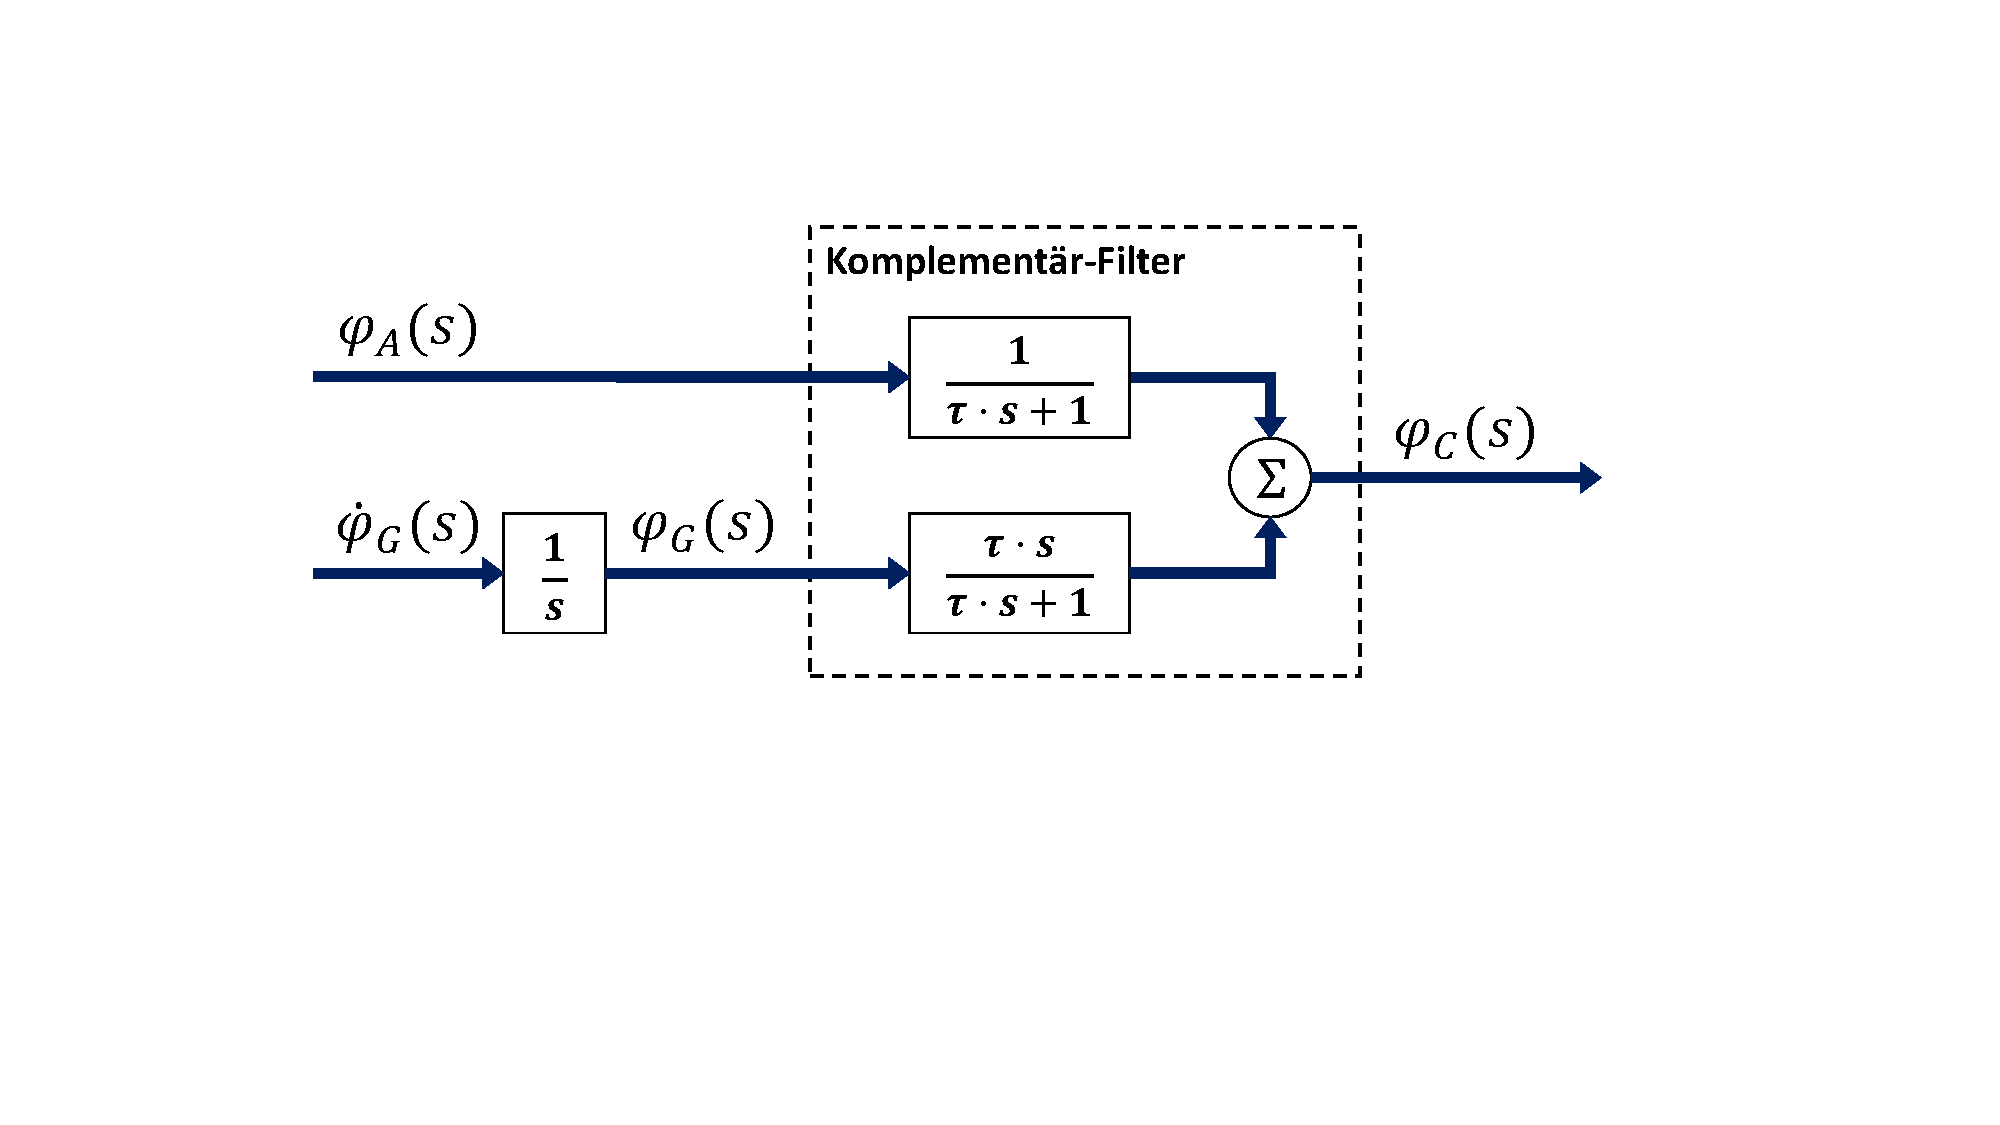
\includegraphics[width=1\linewidth, trim={2cm 7.5cm 4cm 3.5cm}, clip]{img/CompFilter}
\label{bsb_kompfilter}
\caption{Blockschaltbild Komplementärfilter}
\end{figure}

Für das resultierende Signal $\varPhi\idx{C}(s)$ folgt aus dem Blockschaltbild (\ref{bsb_kompfilter})
\begin{equation}
\begin{split}
\varPhi\idx{C}(s) &= \frac{1}{\tau \cdot s + 1}\cdot \varPhi\idx{A}(s) + \frac{\tau \cdot s}{\tau\cdot s + 1}\cdot \varPhi\idx{G}(s)
\\
&= \frac{1}{\tau\cdot s}\cdot \left[\varPhi(s) + V\idx{A}(s)\right] + \frac{\tau\cdot s}{\tau\cdot s + 1}\cdot \left[\varPhi(s) + V\idx{G}(s)\right]
\\
&= \varPhi(s) + \frac{1}{\tau\cdot s}\cdot V\idx{A}(s) + \frac{\tau\cdot s}{\tau\cdot s + 1}\cdot V\idx{G}(s) \,.
\end{split}
\end{equation}
Wird die Zeitkonstante $\tau$ nun so gewählt werden, dass die Störsignale $v\idx{A}$ und $v\idx{G}$ durch das Tief- bzw. Hochpassfilter eliminiert werden, besteht das Ausgangssignal $\varphi\idx{C}$ des Komplementärfilters lediglich aus dem Nutzsignal $\varphi$. Von besonderer Bedeutung für den Regelkreis ist hierbei, dass das Nutzsignal $\varphi$ von keiner Phasenverschiebung betroffen ist.

Dieses Filterkonzept kann auf den Fall des auf einer Ecke stehenden Würfels übertragen werden. Hierbei sind die beiden Winkel $\varphi\idx2$ und $\varphi\idx3$ zu bestimmen. Die Ableitungen dieser Signale hängen von der Winkelgeschwindigkeit $\vel{A}{\omega}{K}$ ab, welche mittels der Drehratensensoren erfasst wird.
\begin{equation}
\begin{bmatrix}
\dot{\varphi}\idx2 \\ \dot{\varphi}\idx3
\end{bmatrix} = \underbrace{\begin{bmatrix}
s_{\varphi\idx3} & c_{\varphi\idx3} & 0
\\
\frac{-s_{\varphi\idx{2}}c_{\varphi\idx{3}}}{c_{\varphi\idx{2}}} & \frac{s_{\varphi\idx{2}}s_{\varphi\idx{3}}}{c_{\varphi\idx{2}}} & 1
\end{bmatrix}}_{\equiv \bs{\Delta\varPhi}}
\cdot 
\begin{bmatrix}
u\idx{K1}\\ u\idx{K2} \\ u\idx{K3}
\end{bmatrix}
\end{equation}
Wird die Matrix $\bs{\Delta\varPhi}$ linearisiert können die Ableitung $\dot{\varphi}\idx2$ und $\dot{\varphi}\idx3$ aus den Winkelgeschwindigkeiten $\bs{u}\idx{K}$ berechnet werden. Die Ergebnisse aus dem vorherigen Abschnitt werden genutzt um die Winkel $\varphi\idx2$ und $\varphi\idx3$ auf den Beschleunigungsmessungen basierend zu schätzen. Mit Hilfe zweier Komplementärfilter werden diese jeweils mit den Ableitungen $\dot{\varphi}_i$ fusioniert. Diese Vorgehensweise führt zu einer ausreichenden Signalgüte um das in Abschnitt (\ref{section_corner_balance_test}) dokumentierten Reglerverhalten zu erreichen. Allerdings zeigt dieser Anwendungsfall die Grenzen des Komplementärfilters auf. Einerseits ist das Filter auf Grund der Linearisierung auf einen lokalen Arbeitsbereich eingeschränkt. Die Linearisierung ist allerdings nötig, da die Ableitungen $\dot{\varphi}_i$ sowohl von den Winkeln $\varphi_i$ als auch den Winkelgeschwindigkeiten $u_{\text{K}i}$ abhängen. Werden für die Berechnung der Matrix $\bs{\Delta\varPhi}$ die Ausgangssignale des Filters verwendet, ergibt sich eine nichtlineare Filteroperation. Des weiteren können die Störsignale $v\idx{A}$ und $v\idx{G}$ durch die Filter nicht vollständig eliminiert werden und beeinflussen somit ebenfalls die Berechnung der Matrix $\bs{\Delta\varPhi}$.
